\documentclass[tikz,12pt]{standalone}
\usepackage{amsmath,amsfonts,amssymb,amsthm}
\usepackage{mathptmx}
\usepackage{tikz}
\usepackage{xcolor}

\definecolor{tblue}{RGB}{25,102,243} % blue
\definecolor{bole}{rgb}{0.8, 0.0, 0.0} % brown
\definecolor{tpink}{rgb}{0.93, 0.23, 0.51} % pink
\definecolor{tgreen}{rgb}{0.0, 0.5, 0.0} % green

\begin{document}
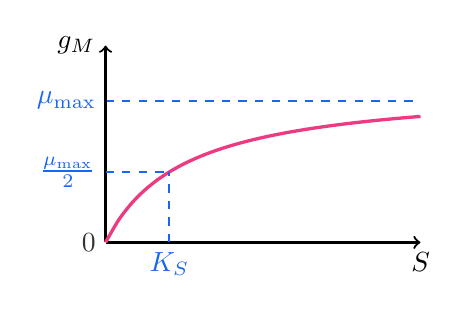
\begin{tikzpicture}
  \draw[tblue, thick, dashed] (0,1.8) --  (4,1.8);
  \node[left,tblue] at (0,1.8) {$\mu_{\max}$};
  \draw[thick, ->,font=\sffamily] (0,0) -- (0,2.5) node[left]{$g_M$};
  \draw[thick, ->] (0, 0) -- (4, 0) node[below]{$S$};
  \node[black!80,left] at (0,0) {$0$};
  \draw[very thick, tpink]   plot[smooth, domain=0:4] (\x,{2*\x/(1+\x)});
  \draw[tblue, thick, dashed] (0.81,0) -- (0.81,0.89);
  \node[below,tblue] at (0.81,0) {$K_S$};
  \draw[tblue, thick, dashed] (0,0.89) -- (0.81,0.89);
  \node[left,tblue] at (0,0.89) {$\frac{\mu_{\max}}{2}$};
\end{tikzpicture}

\end{document}